\documentclass[15pt,a4paper]{article}
\usepackage[portuguese]{babel}
\usepackage[utf8]{inputenc}
\usepackage{indentfirst}
\usepackage{graphicx}
\usepackage{verbatim}
\usepackage{float}
\usepackage{caption}
\usepackage{subcaption}
\begin{document}
\setlength{\textwidth}{16cm}
\setlength{\textheight}{22cm}

\title{\Huge\textbf{Implementação em Prolog do Jogo Oware}\linebreak\linebreak\linebreak
\Large\textbf{Relatório Intercalar}\linebreak\linebreak

\includegraphics[height=6cm, width=7cm]{feup.pdf}\linebreak \linebreak
\Large{Mestrado Integrado em Engenharia Informática e Computação} \linebreak \linebreak
\Large{Programação em Lógica}\linebreak
}

\author{\textbf{Grupo 35:}\\ André Freitas - ei10036 \\ Rui Gonçalves - ei10100 \\\linebreak\linebreak \\
 \\ Faculdade de Engenharia da Universidade do Porto \\ Rua Roberto Frias, s\/n, 4200-465 Porto, Portugal \linebreak\linebreak\linebreak
\linebreak\linebreak\vspace{1cm}}
%\date{Junho de 2007}
\maketitle
\thispagestyle{empty}
\newpage
\section*{Resumo}
Este relatório tem o objetivo de descrever a fase inicial da implementação do Jogo Oware numa linguagem de programação lógica em matemática que é o Prolog. O jogo em questão é de tabuleiro, jogando-se com sementes, sendo muito popular na República do Gana. Apesar da simplicidade das regras tem um forte componente estratégico.

%************************************************************************************************
%************************************************************************************************

%*************************************************************************************************
%************************************************************************************************

\section{Introdução}
Pretende-se explorar as capacidades do Prolog para representar um jogo e as suas regras através deste trabalho. Um jogo é uma excelente maneira de enriquecer o conhecimento na representação e estruturação dos dados bem como a aplicação de regras do jogo traduzidas nesta linguagem. \\
\indent A implementação será em modo de texto, não sendo muito refinada no sentido da apresentação mas sim na componente das funcionalidades. \\
\indent Neste documento pretende-se apresentar a descrição do problema, a representação dos estados do jogo em estruturas conhecidas em Prolog, a representação das jogadas, a visualização do tabuleiro e os apectos de desenvolvimento do projeto.

\section{Descrição do Problema}
O Oware é dos jogos de tabuleiro mais antigos do mundo, tendo sido inventado há mais de 7 mil anos. É jogado por todo o Globo e não existem certezas relativamente à sua origem, porém, atribui-se a sua autoria tradicionalmente ao continente Africano. Atualmente é o jogo mais popular na República do Gana sendo um fenómeno nacional.

\begin{figure}[h!]
\begin{center}
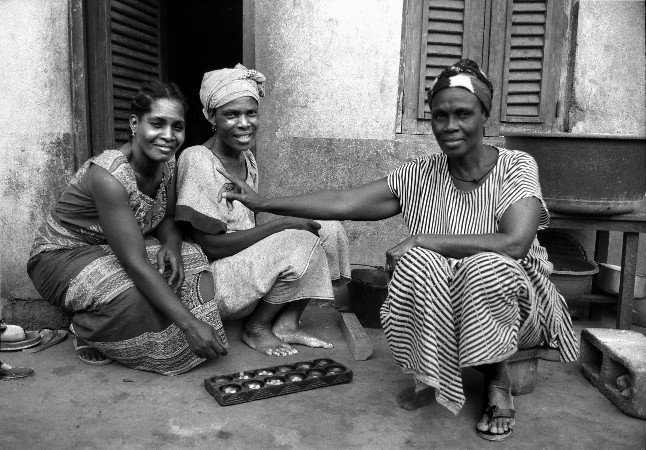
\includegraphics[scale=20]{awale.jpg}
\caption{Pessoas jogando tradicionalmente o Oware}
\label{fig:traditional}
\end{center}
\end{figure}

Como se pode constatar pela Figura 1, existe um tabuleiro com 2x6 cavidades onde se colocam sementes ou feijões. Existem muitas interpretações das regras deste jogo, pelo que iremos adoptar apenas a que é mais conhecida. Assim, o jogo começa com 4 sementes em cada buraco. Os jogadores jogam alternadamente, e em cada jogada tira-se as sementes de um buraco da nossa linha de jogo e vai-se distribuíndo as sementes no sentido anti-horário.
\begin{figure}[H]
\begin{center}
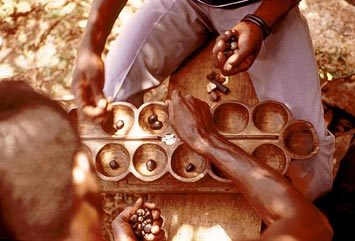
\includegraphics[scale=0.5]{oware.jpg}
\caption{Distribuição das sementes}
\label{fig:peoplePlaying}
\end{center}
\end{figure}
 \indent Quando distribuirmos a última semente e se colocarmos num buraco do adversário e esse sítio ficar com 2 ou 3 sementes, capturamos essas sementes. O jogo termina quando um jogador capturar 25 sementes ou ambos os dois jogadores capturarem 24 sementes (empate).

\subsection{Ilustração de jogadas}
Nas seguintes ilustrações serão descritas duas situações de jogos fundamentais. Pede-se especial atenção para as ilustrações, dado que é necessário estar atento às situações que descrevem para perceber o jogo.\\
\indent Nesta primeira situação o jogo está a começar e o jogador vai distribuir a segunda cavidade de sementes. Assim, as sementes ficaram distribuídas e não houve captura. De notar novamente que o sentido da distribuição das sementes é anti-horário e que o jogador só pode retirar as sementes da sua linha.
\begin{figure} [H]
        \centering
        \begin{subfigure}[f]{0.3\textwidth}
                \centering
                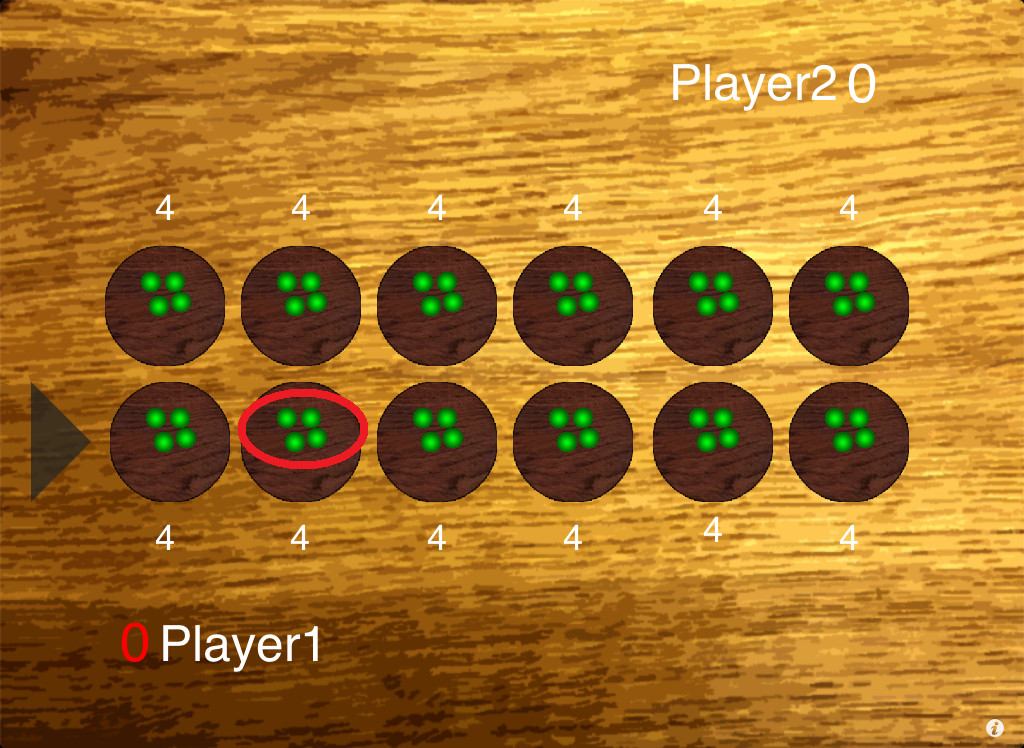
\includegraphics[scale=0.2]{iniciodoJogo.png}
				\caption{Estado Inicial do Jogo}
                \label{fig:inicioJogo}
        \end{subfigure}%
        \quad  \quad
        \begin{subfigure}[f]{0.3\textwidth}
                \centering
                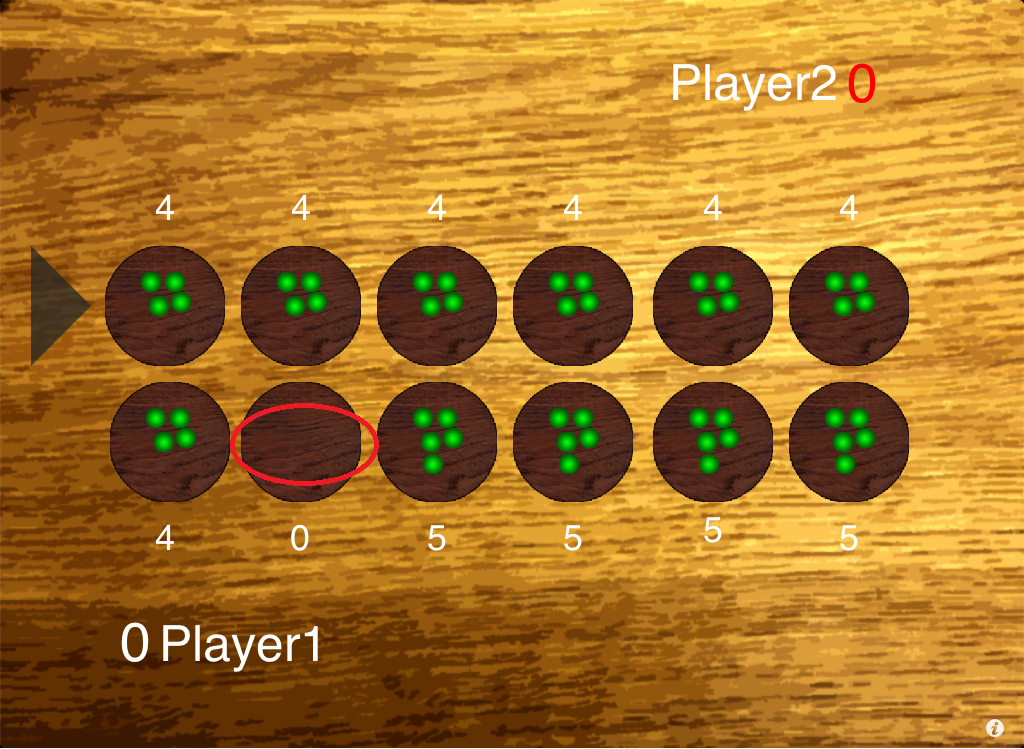
\includegraphics[scale=0.2]{semCaptura.png}
				\caption{Jogada sem Captura}
				\label{fig:semCaptura}
        \end{subfigure}
\end{figure}

A outra jogada importante é a da captura de sementes, ou seja, quando um jogador ao distribuir a última semente calha numa linha do seu adversário, ficam 2 ou 3 sementes nesse sítio, capturando-as. Atenção que se a meio da distribuição das sementes conseguir este número nas cavidades, não as pode capturar, por isso é só na semente final. Destaca-se esta situação dado que existem várias interpretações relativas a esta regra.

\begin{figure} [H]
        \centering
        \begin{subfigure}[f]{0.3\textwidth}
                \centering
                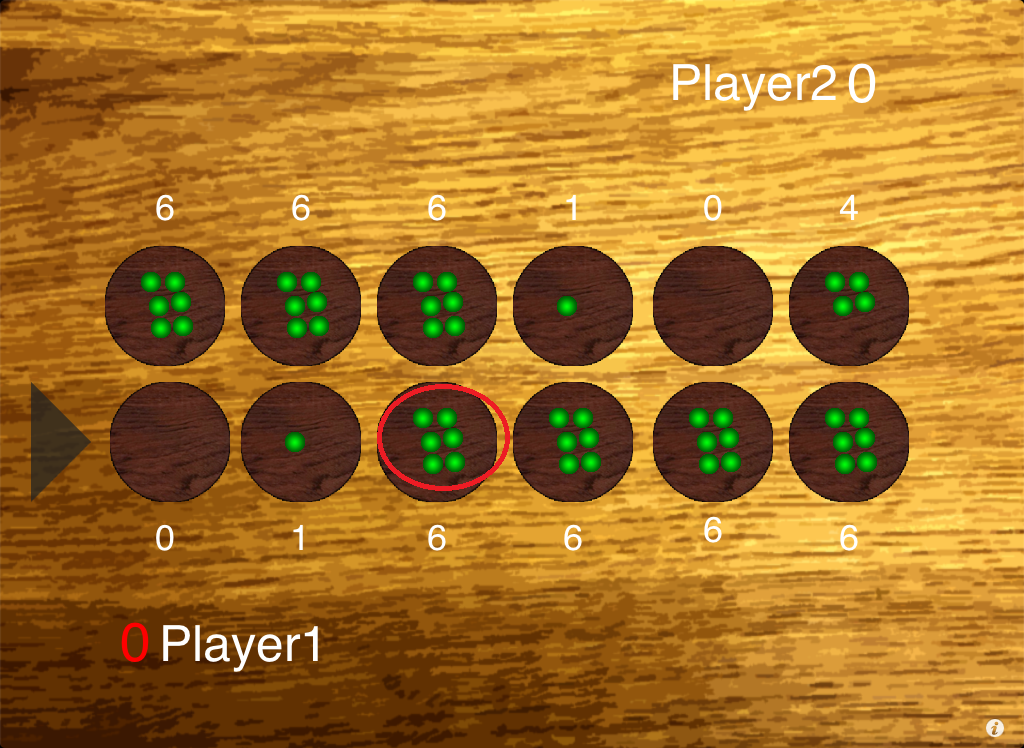
\includegraphics[scale=0.2]{antesCaptura.png}
				\caption{Antes da Captura}
                \label{fig:inicioJogo}
        \end{subfigure}%
        \quad  \quad
        \begin{subfigure}[f]{0.3\textwidth}
                \centering
                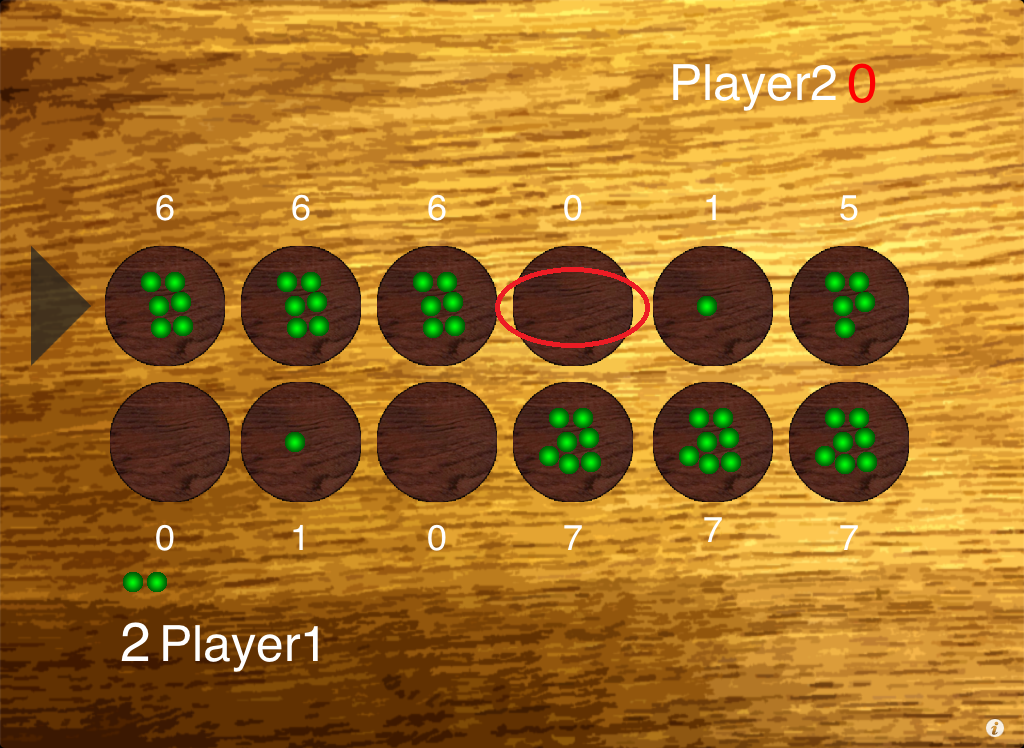
\includegraphics[scale=0.2]{captura.png}
				\caption{Após a Captura de Sementes}
				\label{fig:semCaptura}
        \end{subfigure}
\end{figure}

Pode-se constatar assim a simplicidade do jogo, mas apesar disso requer um componente estratégico para que se possa ganhar, tentando prever-se uma panóplia de jogadas possíveis para vencer o adversário e maximizar as nossas capturas.

\section{Representação do Estado do Jogo}
O tabuleiro é representado por uma lista constituída por duas listas, sendo a primeira a linha do primeiro jogador e a segunda do segundo jogador. De destacar que o tabuleiro é de tamanho constante, apenas variando o valor das sementes em cada posição. O jogo começa com 4 sementes, logo a sua representação no início é:
\begin{center}
\begin{verbatim}
[[4,4,4,4,4,4],[4,4,4,4,4,4]]
\end{verbatim}
\end{center}

\indent Se o jogador 1 (primeira lista) retirar as sementes da posição 0, ao distribuí-las no sentido anti-horário o tabuleiro fica da seguinte maneira:
 \begin{verbatim}
[[0,4,4,4,4,4],[5,5,5,5,4,4]]
\end{verbatim}

\indent No caso de um dos jogadores atingir uma pontuação igual ou superior a 25 esse jogador ganha o jogo pois capturou mais de metade das sementes em jogo, Por exemplo:
 \begin{verbatim}
[[0,5,0,3,0,0],[0,0,0,4,8,4]]
\end{verbatim} 

\indent Num jogo de Oware também é possível, mas pouco provável, empatar pois se os dois jogadores atingirem os 24 pontos todas as sementes em jogo foram capturadas.
 \begin{verbatim}
[[0,0,0,0,0,0],[0,0,0,0,0,0]]
\end{verbatim}

No predicado da Rotina do Jogo, além do estado do tabuleiro, contém também a pontuação de cada jogador.


%-----------------------------------------------------------------------------------
%-----------------------------------------------------------------------------------


\section{Representação de um Movimento}
Tal como constatado anteriormente, o jogo apenas tem uma jogada, que é a distribuição de sementes. Se dessa distribuição resultar na última posição 2 ou 3 sementes é feita uma captura. Assim sendo, existe um predicado para distribuir sementes, que por sua vez chama outro predicado que calcula a sequência de posições para distribuir, alterando depois o tabuleiro e 
verificando se existe possibilidade de captura através de um outro predicado. Após isto, se tiver existido uma captura, os pontos(sementes) do jogador é atualizado.

 \begin{verbatim}
playSeeds(Board,PlayerNum,I,NewBoard)
computeSequence(PlayerNum,I,Seeds,Sequence)
removeSeeds(PlayerNum,[H|[Th|Tt]],I,Seeds,[Hnew|Tnew])
addSeeds(PlayerNum,[H|[Th|Tt]],I,Seeds,[Hnew|Tnew])
evaluateCapture(Board,WhoPlayed,I)
addScore(Score,Val,NewScore)
\end{verbatim}


\section{Visualização do Tabuleiro}
Para a visualização do tabuleiro são usados três predicados: um principal para representar a totalidade do tabuleiro, um para apresentar o logotipo do Jogo e outro para imprimir uma linha de sementes.

 \begin{verbatim}
printBoard([H|[Th|_]],P1Score,P2Score)
printLogo
printBoardLine([H|T])
\end{verbatim}

\begin{figure}[h!]
	\begin{center}
	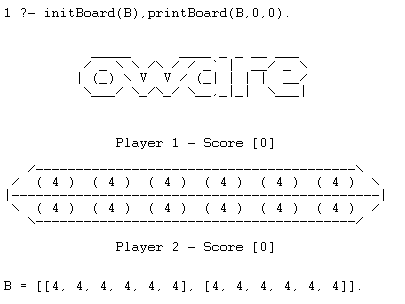
\includegraphics[scale=1]{printBoardExample.png}
	\caption{Começo do jogo}
	\label{fig:Comeco}
	\end{center}
\end{figure}

\section{Conclusões e Perspectivas de Desenvolvimento}
\indent A implementação do Oware em termos de estrutura de dados é simples, porém, 
requer maior esforço na implementação dos predicados que envolvem a distribuição das peças, principalmente o do cálculo da sequência de posições. Existem diversas interpretações das regras e outros nomes para o Oware, por isso tentamos adoptar a versão que é mais conhecida, que já foi aliás implementada em telemóveis.\\

\indent Relativamente ao processo de desenvolvimento de trabalho, iremos adoptar um desenvolvimento iterativo com uma metodologia ágil que é o Scrum. Assim sendo, temos o seguinte Backlog com a estimação dos pontos de esforço, estando ordenado pela prioridade dos itens:

\begin{enumerate}
  \item Representar o tabuleiro numa estrutura [N/A]
  \item Apresentar o tabuleiro em modo de texto [2 pts]
  \item Criar funções básicas para listas [2 pts]
  \item Deve ser possível adicionar e remover sementes na estrutura do tabuleiro [3 pts]
  \item Implementar o cálculo da sequência aquando de uma distribuição de sementes [3 pts]
  \item Implementar um predicado para jogar as sementes [5 pts]
  \item Deve existir um predicado que avalia se há uma captura, devolvendo a posição das sementes [5 pts]
  \item Implementar um predicado para ler o input do teclado [2 pts]
  \item Implementar a rotina de jogo [8 pts]
  \item Deve existir um bot que a deva conseguir determinar que posição das sementes deve jogar a partir da linha do adversário [8 pts]
\end{enumerate}

Ora assumindo este Backlog e tendo em conta que já implementamos até ao quarto item falta 80\% do esforço deste trabalho, usando uma estimativa mais razoável. Tento em conta isto, não se traduz em horas de trabalho mas sim esforço e ultrapassar dificuldades. Os pontos mais críticos serão a rotina de jogo e a implementação da inteligência artificial do Bot.

\clearpage
\addcontentsline{toc}{section}{Bibliografia}
\renewcommand\refname{Bibliografia}
\bibliographystyle{plain}
\bibliography{myrefs}

\newpage
\appendix
\section{Código Implementado}
 \begin{verbatim}
% Starts the board with the default seeds
initBoard([[4,4,4,4,4,4],[4,4,4,4,4,4]]).

% Board Visualization
% Test with: initBoard(B),printBoard(B,0,0).
printBoardLine([]).
printBoardLine([H|T]):-
	write(' ( '),
	write(H),
	write(' ) '),
	printBoardLine(T).

printLogo:-
	write('\n\n'),
	write('           _____      ____ _ _ __ ___\n'), 
	write('          / _ \\ \\ /\\ / / _` |  __/ _ \\ \n'),
	write('         | (_) \\ V  V / (_| | | |  __/ \n'),
	write('          \\___/ \\_/\\_/ \\__,_|_|  \\___| \n\n\n').
	
printBoard([H|[Th|_]],P1Score,P2Score):-
	printLogo,
	write('\n'),
	write('              Player 1 - Score ['),
	write(P1Score),
	write(']\n\n'),
	write('   /----------------------------------------\\ \n'),
	write(' / '), printBoardLine(H),write(' \\ \n'),
	write('|----------------------------------------------|'),
	write('\n \\ '), printBoardLine(Th), write(' / \n'),
	write('   \\----------------------------------------/\n\n'),
	write('              Player 2 - Score ['),
	write(P2Score),
	write(']\n\n\n').
	

% List Core Functions
replace([_|T],0,X,[X|T]).
replace([H|T],N,X,[H|T2]):- 
	N>0, 
	N1 is N-1,
	replace(T,N1,X,T2).

element([H|T],0,H).
element([_|T],N,Val):-
	N>0,
	N2 is N-1,
	element(T,N2,Val).

elementPlus(List,I,Value,NewList):-
	element(List,I,Oldval),
	Newval is Oldval+Value,
	replace(List,I,Newval,NewList).
	
elementMinus(List,I,Value,NewList):-
	element(List,I,Oldval),
	Newval is Oldval-Value,
	replace(List,I,Newval,NewList).

% In game functions
initScore(0).
addScore(Score,Val,NewScore):-NewScore is Score+Val.

addSeeds(PlayerNum,[H|[Th|Tt]],I,Seeds,[Hnew|Tnew]):-
	PlayerNum=1,
	elementPlus(H,I,Seeds,Hnew),
	Tnew = [Th|Tt];
	PlayerNum=2,
	elementPlus(Th,I,Seeds,Tnew),
	Hnew = H.
	
removeSeeds(PlayerNum,[H|[Th|Tt]],I,Seeds,[Hnew|Tnew]):-
	PlayerNum=1,
	elementMinus(H,I,Seeds,Hnew),
	Tnew = [Th|Tt];
	PlayerNum=2,
	elementMinus(Th,I,Seeds,Tnew),
	Hnew = H.
		
% To implement later
%computeSequence(PlayerNum,I,Seeds,Sequence)
%playSeeds(Board,PlayerNum,I,NewBoard)
%evaluateCapture(Board,WhoPlayed,I)
%gameRoutine(Board,Player1Score,Player2Score):

gameRoutine(_,25,_).
gameRoutine(_,_,25).
gameRoutine(_,24,24).

\end{verbatim}
\end{document}
